% !TeX root = ../tfg.tex
% !TeX encoding = utf8

\chapter{Símplices y complejos simpliciales}

Los espacios topológicos pueden llegar a ser complicados de estudiar. Los complejos simpliciales tienen la ventaja de ser estructuras fáciles de estudiar y definiéndolos en cierta forma como espacios topológicos admiten homeomorfismos a un gran número de espacios topológicos. En este capítulo nos centraremos en la definición y el estudio de estos objetos en profundidad en la línea de \cite{munkres2018elements} y lo complementaremos con alguna aportación de \cite{lee2010introduction}.

\section{Símplices}

Con la finalidad de generalizar estructuras como el triángulo y el tetraedro, 
a finales del siglo XIX nace un nuevo concepto: el símplice. Su sencillez y 
propiedades lo convirtieron en una herramienta muy versátil en el estudio de la
topología algebraica, dando lugar a lo que hoy conocemos como homología simplicial. 
En esta sección definiremos lo que es un símplice y algunos conceptos asociados a él
que nos serán de gran utilidad en el estudio de dicho campo. Comenzamos recordando algunos conceptos de la geometría afín.

Como tan sólo será necesario trabajar en el espacio afín usual $N$-dimensional, lo notaremos simplemente por $\mathbb{R}^{N}$.

\begin{definicion}
	Sea $\{a_0, \dots, a_p\}$ un conjunto de puntos en $\mathbb{R}^N$. 
	Diremos que dicho conjunto es \textbf{afínmente independiente} si 
	para cualesquiera $t_i \in \mathbb{R}$, las ecuaciones
	\[ \sum_{i=0}^{p}t_i=0 \quad \text{y} \quad \sum_{i=0}^{p}t_ia_i=0 \]
	implican que $t_0 = t_1 = \dots = t_p$.
\end{definicion}

\begin{definicion}
	Sea $\{a_0, \dots, a_p\}$ un conjunto de puntos afínmente independiente. 
	Definimos el \textbf{plano afín} $P$ generado por $\{a_0, \dots, a_p\}$ como
	el conjunto de puntos $x \in \mathbb{R}^N$ tales que
	\[ x = \sum_{i=0}^{p}t_ia_i = a_0 + \sum_{i=1}^{p}t_i(a_i - a_0) \]
	para algunos $t_1, \dots, t_p \in \mathbb{R}$. Diremos entonces que $P$ es el 
	plano que pasa por $a_0$ paralelo a los vectores $a_i - a_0$, $i \in \{1, \dots, p\}$.
\end{definicion}

Nótese que la transformación afín $T$ de $\mathbb{R}^N$ tal que $T(x) = x - a_0$ es una traslación que lleva el plano $P$ al subespacio vectorial de $\mathbb{R}^N$ con base $a_1-a_0, a_2-a_0, \dots, a_p-a_0$. Si componemos dicha transformación con una aplicación lineal que lleve cada vector $a_1-a_0, a_2-a_0, \dots, a_p-a_0$ a los primeros $N$ vectores de la base usual, obtenemos una transformación afín $S: P \rightarrow \R^N \times \{0\}$ tal que $S(a_i) = (0, \overset{i-1}{\dots}, 0, 1, 0, \overset{i+1}{\dots}, 0)$ con $i \in \{1, \dots, p\}$.

\begin{definicion}
	Sea $\{a_0, \dots, a_p\}$ un conjunto de puntos afínmente independiente en 
	$\mathbb{R}^N$. Definimos el \textbf{p-símplice} o \textbf{símplice} $\sigma = [a_0, \dots, a_p]$ 
	generado por $a_0, 	\dots, a_p$ como el conjunto de todos los $x \in \mathbb{R}^N$ 
	tales que
	\[ x=\sum_{i=0}^{p}t_ia_i \quad \text{y} \quad \sum_{i=0}^{p}t_i=1 \]
	con $t_i \geq 0$, $i \in \{1, \dots, p\}$.
\end{definicion}
\begin{definicion}
	Sea $\sigma$ un $p$-símplice. A los términos $t_0, \dots, t_p$ los llamamos las \textbf{coordenadas baricéntricas} de $\sigma$
	con respecto a $a_0, \dots, a_p$.
\end{definicion}

\begin{proposicion}
	Sea $\sigma=[a_0,a_1,\dots,a_p]$ un $p$-símplice. Entonces las coordenadas baricéntricas de cualquier $x \in \sigma$ están determinadas de manera única.
\end{proposicion}
\begin{proof}
	Sea $y \in \sigma$ un punto arbitrario del $p$-símplice en $\R^N$. Como hemos definido nuestro símplice como combinación convexa de los puntos $a_0, a_1, \dots, a_p$ tenemos que dichas coordenadas existen (además de ser no negativas) y son solución de la siguiente ecuación
	\[
	Ax = \begin{pmatrix}
		a_{01} & a_{02} & \cdots  & a_{0p} \\
		a_{11} & a_{12} & \cdots & a_{1p} \\
		 \vdots & \vdots & \ddots & \vdots \\
		a_{N1} & a_{N2} & \cdots & a_{Np}  \\
		1 & 1 & 1 & 1 
	\end{pmatrix}
	\begin{pmatrix}
		t_0 \\
		t_1 \\
		\vdots \\
		t_p
	\end{pmatrix}
	= 
	\begin{pmatrix}
		y_0 \\
		y_1 \\
		\vdots \\
		y_p
	\end{pmatrix}
	\]
	donde $a_i = (a_{0i}, \dots, a_{Ni})^T$ con $0 \leq i \leq p$, $x = (t_0,t_1,\dots,t_p)^T$ e $y = (y_0,y_1,\dots,y_p)^T$. El superíndice $T$ indica la matriz traspuesta. 
	
	En cuanto a la unicidad, basta suponer la existencia de otro $x'=(t_0',t_1', \dots, t_p')^T$ tal que $Ax = y = Ax'$. Sin embargo, dicha igualdad se cumple si, y sólo si, $A(x-x')=0$. Como $a_0,a_1,\dots,a_p$ son afínmenente independientes, tenemos que el determinante de $A$ no puede ser $0$ y por tanto $A$ no puede ser la matriz nula. Nos queda que $x-x'=0$ debe cumplirse luego $x=x'$.
\end{proof}

Los puntos $a_0, \dots, a_p$ que generan $\sigma$ los llamaremos \textbf{vértices} de $\sigma$
y al número $p$ lo llamaremos la \textbf{dimensión} de $\sigma$.

\begin{definicion}
	Sea $\sigma=[a_0, \dots, a_p]$ un símplice. Una \textbf{cara de dimensión $p$} de $\sigma$ será cualquier
	símplice generado por un subconjunto no vacío de $\{a_0, \dots, a_p\}$.
\end{definicion}
En particular, la cara de $\sigma$ generada por $a_0, \dots, a_{i-1}, a_{i+1}, \dots, a_p$ la 
llamamos la \textbf{cara opuesta} de $a_i$, $i \in \{0, \dots, p\}$. Las caras de $\sigma$ 
diferentes de $\sigma$ diremos que son \textbf{caras propias} de $\sigma$ y la unión de todas ellas la 
llamaremos el \textbf{borde} de $\sigma$ y lo notaremos $\text{Bd}\ \sigma$. Finalmente, definimos el \textbf{interior} de $\sigma$, $\text{Int}\ \sigma$, como el conjunto de puntos de $\sigma$ que no pertenecen 
a su borde.

\begin{figure}[h]
	\begin{subfigure}{.24\textwidth}
		\centering
		
\begin{tikzpicture}
			% 3-símplice
			\node (n0) at (0.0,  0.0) {}; % root
			
			% DRAW NODES
			\draw[color=black, fill=black] (n0) circle (.1);
		\end{tikzpicture}
		\caption{0-símplice}
	\end{subfigure}
	\hfill
	\begin{subfigure}{.24\textwidth}
		\centering
		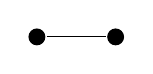
\begin{tikzpicture}
			% 3-símplice
			\node (n0) at (0.0,  0.0) {}; % root
			\node (n1) at (1.0, 0.0) {}; % extreme
			
			% DRAW TREE
			\path[draw] (n0)--(n1);
			
			% DRAW NODES
			\draw[color=black, fill=black] (n0) circle (.1);
			\draw[color=black, fill=black]  (n1) circle (.1);
		\end{tikzpicture}
		\caption{1-símplice}
	\end{subfigure}
	\hfill
	\begin{subfigure}{.24\textwidth}
		\centering
		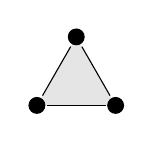
\begin{tikzpicture}
			% 3-símplice
			\node (n0) at (0.0,  0.0) {}; % root
			\node (n1) at (1.0, 0.0) {}; % extreme
			\node (n2) at (0.5, 0.87) {}; % extreme
			
			% DRAW TREE
			\fill[fill=gray!20] (n0.center)--(n1.center)--(n2.center);
			\path[draw] (n0)--(n1);
			\path[draw] (n1)--(n2);
			\path[draw] (n2)--(n0);
			
			% DRAW NODES
			\draw[color=black, fill=black] (n0) circle (.1);
			\draw[color=black, fill=black]  (n1) circle (.1);
			\draw[color=black, fill=black]  (n2) circle (.1);
		\end{tikzpicture}
		\subcaption{2-símplice}
	\end{subfigure}
	\hfill
	\begin{subfigure}{.24\textwidth}
		\centering
		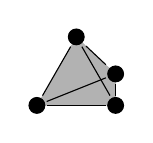
\begin{tikzpicture}
			% 3-símplice
			\node (n0) at (0.0,  0.0) {}; % root
			\node (n1) at (1.0, 0.0) {}; % extreme
			\node (n2) at (0.5, 0.87) {}; % extreme
			\node (n3) at (1.0, 0.4) {}; % inside
			
			% DRAW TREE
			\fill[fill=gray!60] (n0.center)--(n1.center)--(n2.center);
			\fill[fill=gray!60] (n0.center)--(n2.center)--(n3.center);
			\fill[fill=gray!60] (n0.center)--(n1.center)--(n3.center);
			\fill[fill=gray!60] (n3.center)--(n1.center)--(n2.center);
			\path[draw] (n0)--(n1);
			\path[draw] (n1)--(n2);
			\path[draw] (n2)--(n0);
			\path[draw] (n0)--(n3);
			\path[draw] (n1)--(n3);
			\path[draw] (n2)--(n3);
			
			% DRAW NODES
			\draw[color=black, fill=black] (n0) circle (.1);
			\draw[color=black, fill=black]  (n1) circle (.1);
			\draw[color=black, fill=black]  (n2) circle (.1);
			\draw[color=black, fill=black]   (n3) circle (.1);
		\end{tikzpicture}
		\caption{3-símplice}
	\end{subfigure}
	\caption{Símplices de dimensión $0$, $1$, $2$ y $3$}
	\label{fig:simplex}
\end{figure}

Dado un símplice $\sigma$ podemos definir un orden sobre sus vértices. Dos órdenes de $\sigma$ los consideraremos equivalentes si podemos pasar de uno a otro con un número par de permutaciones. Así, los ordenamientos posibles para los vértices de $\sigma$ se pueden agrupar en dos clases de equivalencia distintas, que definimos como las \textbf{orientaciones del símplice} $\sigma$.

\begin{definicion}
Decimos que un símplice $\sigma = [a_0, a_1, \ldots, a_p]$ está \textbf{orientado} si se le ha asignado una de estas orientaciones. Utilizaremos $[a_0 a_1 \ldots a_p]$ para denotar la clase de equivalencia dada por la orientación $a_0 < a_1 < \cdots < a_p$ del símplice generado por los vértices $a_0,a_1,\ldots, a_p$.
\end{definicion}

\section{Complejos simpliciales}

La importancia de los complejos simpliciales reside en su capacidad para descomponer espacios topológicos en componentes manejables, permitiendo un análisis detallado de su estructura. Al considerar la forma en que estos símplices se conectan y orientan entre sí, los complejos simpliciales facilitarán la definición de cadenas y ciclos simpliciales que serán indispensables en el estudio de la homología simplicial.

\begin{definicion}
	Un \textbf{complejo simplicial} $K$ en $\mathbb{R}^N$ es una colección de símplices en $\mathbb{R}^N$
	 tal que:
	\begin{enumerate}
		\item Toda cara de un símplice de $K$ está en $K$.
		\item La intersección de cualesquiera dos símplices de $K$ es una cara 
		de ambos símplices.
	\end{enumerate}
\end{definicion}

En ciertas ocasiones puede ser interesante saber si dada una colección cualquiera de símplices, esta es 
un complejo simplicial o no. Para ello, el siguiente lema nos puede ser de utilidad.

\begin{lema}
	Una colección $K$ de símplices es un complejo simplicial si, y sólo si, se cumplen las siguientes 
	condiciones:
	\begin{enumerate}
		\item Toda cara de un símplice de $K$ está en $K$.
		\item La intersección dos a dos del interior de los símplices de $K$ es disjunta.
	\end{enumerate}
\end{lema}
\begin{proof}
	Primero, asumamos que $K$ es un complejo simplicial. Dados dos símplices $\sigma, \tau \in K$ veamos que si el interior de ambos tiene un punto $x$ en común, entonces $\sigma = \tau$. Sea $s = \sigma \cap \tau$ y considero $x \in s$. Si $s$ fuera una cara propia de $\sigma$, entonces $x$ pertenecería a la frontera de $\sigma$, lo cual no se cumple ya que $x$ pertenece al interior de $\sigma$. Por tanto $s = \sigma$. De manera análoga, $s = \tau$, luego $\sigma = \tau$.
	
	Asumamos ahora que se cumplen \textit{(1)} y \textit{(2)}. Queremos ver que si el conjunto $\sigma \cap \tau \neq \emptyset$,  dicha intersección es la cara $\sigma'$ de $\sigma$ generada por los vértices $b_0,\dots,b_m$ de $\sigma$ que están en $\tau$. Primero, $\sigma' \subset \sigma \cap \tau$ por ser $\sigma \cap \tau$ convexa y contener a $b_0, \dots, b_m$. Para la otra inclusión supongamos que $x \in \sigma \cap \tau$. Esto implica que $x \in \text{Int}\ s \cap \text{Int}\ t$ para alguna cara $s$ de $\sigma$ y alguna cara $t$ de $\tau$. Se sigue de \textit{(2)} que $s = t$ por lo que los vértices de $s$ están en $\tau$ y por definición, son elementos del conjunto $\{b_0, \dots, b_m\}$.  Concluimos entonces que $s$ es una cara de $\sigma'$, lo que implica que $x \in \sigma'$, como queríamos ver.
\end{proof}

\begin{definicion}
	Si $L$ es una subcolección del complejo simplicial $K$ que contiene todas las caras de sus 
	elementos, entonces $L$ es un complejo simplicial que llamaremos \textbf{subcomplejo} de $K$.
\end{definicion}
Entre los subcomplejos de un complejo simplicial, cabe destacar el siguiente. Diremos \textbf{p-esqueleto} 
de $K$ al subcomplejo formado por todas las caras de $K$ cuya dimensión sea menor o igual que $p$. Lo denotaremos por $K^{(p)}$. En particular, $K^{(0)}$ lo llamaremos el \textbf{conjunto de vértices} de $K$.

\begin{definicion}
	Sea $K$ un complejo simplicial de $\mathbb{R}^N$ y sea $|K|$ el subconjunto de $\mathbb{R}^N$ tal que $|K|$ es la unión de todos los símplices de $K$. Definimos el \textbf{politopo} o \textbf{espacio subyacente} 
	de $K$ como el espacio topológico $(|K|, \mathcal{T})$ donde los abiertos de $\mathcal{T}$ son aquellos $O \subseteq |K|$ tal que $O \cap \sigma$ es abierto en $\sigma$ con la topología inducida de $\mathbb{R}^N$ para todo $\sigma \in K$.
\end{definicion}

Veamos que en efecto $(|K|, \mathcal{T})$ es un espacio topológico. $\emptyset, |K| \in \mathcal{T}$ ya que son abiertos trivialmente en $\sigma$, pues $\emptyset \cap \sigma = \emptyset$ y $|K| \cap \sigma = \sigma$ para todo $\sigma \in K$. Si $O_1, O_2 \in \mathcal{T}$, entonces $O_1 \cap \sigma$, $O_2 \cap \sigma$ son abiertos en $\sigma$ luego $(O_1 \cap O_2) \cap \sigma = (O_1 \cap \sigma) \cap (O_2 \cap \sigma)$ es abierto en $\sigma$ para todo $\sigma \in K$. Por tanto $O_1 \cap O_2 \in \mathcal{T}$. Finalmente, consideremos una familia $\{O_i\}_{i \in I} \subset \mathcal{T}$ donde $I$ es un conjunto de índices. Para cada $\sigma \in K$, $(\cup_{i \in I} O_i) \cap \sigma = \cup_{i \in I} (O_i \cap \sigma)$ que efectivamente es una unión arbitraria de abiertos de $\sigma$. En consecuencia, $\cup_{i \in I} O_i \in \mathcal{T}$.

En general, la topología de $|K|$ es más fina que la inducida de la topología usual de $\R^N$. Si $A$ es cerrado en $|K|$ con la topología inducida de la usual, $A=B \cap |K|$ para algún cerrado $B$ de $\R^N$ y por tanto $B \cap \sigma$ sería cerrado en $\sigma$ para cada símplice $\sigma$ de $K$. Como consecuencia, $B \cap |K|=A$ es cerrado en $|K|$ con la topología $\mathcal{T}$ definida anteriormente. 

Si no hay lugar a confusión, simplemente notaremos al politopo de $K$ por $|K|$ y lo llamaremos el \textbf{poliedro} $|K|$.

\begin{lema}\label{lem:cont_poly}
	Sea $K$ un comlpejo simplicial y $X$ un espacio topológico. Una aplicación $f: |K| \rightarrow X$ es continua si, y sólo si, $f|_{\sigma}$ es continua para cada $\sigma \in K$.
\end{lema}
\begin{proof}
	Si $f$ es continua, también lo es $f|_{\sigma}$ por ser $\sigma$ un subespacio de $K$. Supongamos ahora que $f|_{\sigma}$ es continua para cada $\sigma \in K$. Si $C$ es un cerrado de $X$, $f^{-1}(C) \cap \sigma = f|_{\sigma}^{-1}(C)$ es un cerrado en $\sigma$ por la continuidad de $f|_{\sigma}$. Concluimos que $f^{-1}(C)$ es cerrado en $|K|$ por definición.
\end{proof}

\begin{definicion}
	Un espacio topológico $X$ es \textbf{triangulable} si existe un complejo simplicial $K$ cuyo espacio subyacente es homeomorfo a $X$. Diremos entonces que el homeomorfismo $h: |K| \rightarrow X$ es una \textbf{triangulación}.
\end{definicion}

\section{Aplicaciones simpliciales}

Cuando trabajemos con complejos simpliciales, será interesante tener en cuenta cuándo las 
transformaciones entre ellos pueden ser continuas o incluso homeomorfismos. 

\begin{lema}
	Sean $K$ y $L$ dos complejos simpliciales y sea $f: K^{(0)} \rightarrow L^{(0)}$ una aplicación entre los conjuntos de vértices de $K$ y $L$. 
	Supongamos que siempre que los vértices $v_0, \dots, v_n$ de $K$ generen un símplice en $K$, 
	los puntos $f(v_0), \dots, f(v_n)$ son vértices de un símplice de $L$. Entonces podemos extender $f$ 
	a una aplicación continua $g:|K| \rightarrow |L|$ tal que
	\[ x = \sum_{i=0}^{n}t_iv_i \quad \implies \quad g(x) = \sum_{i=0}^{n}t_if(v_i) \]
	Llamaremos a $g$ la \textbf{aplicación simplicial} (lineal) inducida por $f$.
\end{lema}

\begin{proof}
	Por hipótesis, los vértices $f(v_0), \dots, f(v_n)$ generan un símplice $\tau$ en $L$. Por 
	ser $K$ un complejo simplicial, la suma de sus coeficientes $t_i$, con $i \in \{0, \dots, n\}$,  
	es igual a uno, luego $g(x) = \sum_{i=0}^{n}t_if(v_i)$ es un punto de $\tau$. Podemos ver que 
	$g$ es una aplicación continua del símplice $\sigma$ generado por $v_0, \dots, v_n$ al símplice 
	$\tau$ generado por $f(v_0), \dots, f(v_n)$.
	
	Ahora tan solo nos queda ver que $g:|K| \rightarrow |L|$ es continua. Bien, pues por ser 
	$g: \sigma \rightarrow \tau$ continua, también lo es $g: \sigma \rightarrow |L|$. Finalmente 
	por el \autoref{lem:cont_poly}, $g:|K| \rightarrow |L|$ es continua.
\end{proof}

\begin{lema}\label{lem:homeo_complex}
	Supongamos que $f:K^{(0)} \rightarrow L^{(0)}$ es una aplicación biyectiva tal que los vértices 
	$v_0, \dots, v_n$ de $K$ generan un símplice de $K$ si, y sólo si, $f(v_0), \dots, f(v_n)$ 
	generan un símplice de $L$. Entonces la aplicación simplicial inducida $g:|K| \rightarrow |L|$ 
	es un homeomorfismo. Diremos entonces que $g$ es un \textbf{homeomorfismo simplicial} de $K$ con $L$.
\end{lema}

\begin{proof}
	Por hipótesis, cada símplice $\sigma \in K$ se identifica con otro símplice $\tau \in L$. 
	Por tanto, debemos comprobar que la aplicación lineal $h: \tau \rightarrow \sigma$ inducida por 
	la correspondencia de vértices $f^{-1}$ es la inversa de $g: \sigma \rightarrow \tau$. Si 
	consideramos $x = \sum_{i=0}^{n}t_i v_i$, entonces por definición $g(x) = \sum_{i=0}^{n}t_if(v_i)$.
	Luego
	\[ h(g(x)) = h(\sum_{i=0}^{n}t_if(v_i)) = \sum_{i=0}^{n}t_i f^{-1}(v_i) = \sum_{i=0}^{n}t_i v_i = x \]
\end{proof}

\section{Complejos simpliciales abstractos}

Si bien la definición actual de los complejos simpliciales puede llegar a ser de gran utilidad, en 
la práctica muchas veces no es necesario usar las herramientas que nos proporciona la geometría afín. 
Es por ello que vamos a introducir una descripción puramente combinatoria de los complejos simpliciales 
que, aun siendo más simple, nos serán de gran utilidad a la hora de trabajar con espacios topológicos.

\begin{definicion}
	Un \textbf{complejo simplicial abstracto} (o simplemente complejo abstracto) es una 
	colección $\mathcal{S}$ de conjuntos finitos no vacíos tal que si $A \in \mathcal{S}$, 
	entonces para todo $B \subset A$ con $B$ no vacío, $B \in \mathcal{S}$.
\end{definicion}

Al elemento $A$ de $\mathcal{S}$ lo llamaremos \textbf{símplice} de $A \in \mathcal{S}$. La 
\textbf{dimensión} de $A$ es una menos que el número de elementos que le pertenecen. Todo 
subconjunto de $A$ lo llamaremos \textbf{cara} de $A$. En cuanto a la \textbf{dimensión} de 
$\mathcal{S}$, diremos que es igual al máximo de las dimensiones de sus elementos o en caso de 
no haberlo, diremos que la dimensión de $\mathcal{S}$ es infinita. El \textbf{conjunto de vértices} 
$V$ de $\mathcal{S}$ diremos que es la unión de elementos de $\mathcal{S}$ que contienen un único punto. 
Llamaremos \textbf{subcomplejo} de $\mathcal{S}$ a cualquier subcolección de $\mathcal{S}$ que sea 
un complejo simplicial abstracto en sí.

Sean $V_S$, $V_T$ los conjuntos de vértices de los complejos abstractos $\mathcal{S}$, $\mathcal{T}$  respectivamente. Dos complejos abstractos $\mathcal{S}$ y $\mathcal{T}$ diremos que son 
\textbf{isomorfos} si existe una aplicación biyectiva $f: V_S \rightarrow V_T$ tal que 
$\{a_0, \dots, a_p\} \in \mathcal{S}$ si, y sólo si, $\{f(a_0), \dots, f(a_p)\} \in \mathcal{T}$.

\begin{definicion}
	Sean $K$ un complejo simplicial y $V$ su conjunto de vértices. Sea $\mathcal{K}$ la colección de 
	todos los subconjuntos $\{a_0, \dots, a_p\} \subset V$ tales que los vértices $a_0, \dots, a_p$ 
	generan un símplice de $K$. Entonces llamaremos a la colección $\mathcal{K}$ el 
	\textbf{esquema de vértices} de $K$.
\end{definicion}

Después de realizar todas las definiciones pertinentes, ya estamos en condiciones de enunciar el 
siguiente teorema.

\begin{teorema}
	Las siguientes afirmaciones son ciertas:
	\begin{enumerate}[label=(\alph*)]
		\item Todo complejo abstracto $\mathcal{S}$ es isomorfo al esquema de vértices de algún 
		complejo simplicial $K$.
		\item Dos complejos simpliciales son afínmente isomorfos si, y sólo si, sus esquemas 
		de vértices son isomorfos como complejos simpliciales abstractos.
	\end{enumerate}
\end{teorema}
\begin{proof}
	Para demostrar $(a)$, empezaremos tomando un conjunto de índices $J$. Llamemos $\mathbf{E}^J$ 
	al subconjunto de funciones $x: J \rightarrow \mathbb{R}$ de $\mathbb{R}^J$ tales que $x(\alpha) = 0$ 
	para todo $\alpha \in J$ excepto para un número finito de valores. Sea $\Delta^J$ la 
	colección de todos los símplices en $\mathbf{E}^J$ generados por subconjuntos finitos de 
	la base usual de $\mathbf{E}^J$. $\Delta^J$ es un complejo simplicial. 
	Sean entonces $\sigma, \tau$ símplices de $\Delta^J$, la 
	unión de sus conjuntos de vértices es afínmente independiente y genera un símplice en $\Delta^J$.
	Diremos que $\Delta^J$ es un \textbf{símplice de dimensión infinita}.
	
	Sea ahora $\mathcal{S}$ un complejo abstracto con conjunto de vértices $V$. Tomamos un conjunto 
	de índices $J$ lo bastante grande para que podamos tomar una aplicación inyectiva 
	$f: V \rightarrow J$. A continuación, vamos a tomar un subcomplejo de $\Delta^J$ tal que para 
	cada símplice abstracto $\{a_0, \dots, a_p\} \in \mathcal{S}$, el símplice (geométrico) generado 
	por $f(a_0), \dots, f(a_p)$ está en $K$. Por tanto $K$ es un complejo simplicial y 
	$f$ es un isomorfismo entre $\mathcal{S}$ y el esquema de vértices de $K$.
	
	En cuanto a $(b)$, es una consecuencia inmediata del \autoref{lem:homeo_complex}.
\end{proof}

\begin{definicion}
	Si el complejo simplicial abstracto $\mathcal{S}$ es isomorfo al esquema de vértices del 
	complejo simplicial $K$, diremos que $K$ es una \textbf{realización geométrica} de $\mathcal{S}$.
\end{definicion}

%\begin{ejemplo}
%	Supongamos que queremos encontrar un complejo simplicial $K$ que sea homeomorfo al cilindro $S^1 \times [0,1]$. Una forma de hacerlo sería definiendo $K$ como una colección de 6 $2-$símplices y sus caras tal y como se puede apreciar en la FIGURA ??. Otra forma sería definir un complejo simplicial $L$ cuyo espacio subyacente sea un rectángulo dotado de una serie de vértices  
%\end{ejemplo}

\endinput
%--------------------------------------------------------------------
% FIN DEL CAPÍTULO. 
%--------------------------------------------------------------------
